%%%%%%%%%%%%%%%%%%%%%%%%%%%%%%%%%%%%%%%%%%%%%%%%%%%%%%%%%%%%%%%%
%%%%%%%%%%%%%%%%%%%%%%%%%%%%%%%%%%%%%%%%%%%%%%%%%%%%%%%%%%%%%%%%
%%%%%%%%%%%%%%%%%%%%%%%%%%%%%%%%%%%%%%%%%%%%%%%%%%%%%%%%%%%%%%%%

\eglabel{6}
\section{Example \theexamples: Joint PKPD model with count data}
\label{sec:eg6}
The following three examples features a new aspect of the \pml, the support of discrete 
data models\footnote{The discrete data models are coming in a large variety, which 
would be worth a detailed discussion. This and the next examples can cover, for 
the sake of space, only the very basic cases. More examples, encoded completely 
in \pml, can be found on our webpage \url{http://pharmml.org}. See also discrete data 
model templates in the appendix, \ref{chapter:codeTemplates}.}. The first one is using 
the Poisson distribution to describe count data\footnote{The example is encoded 
in \xatt{example6\_NONMEM.xml} with design sourced from a NONMEM datafile.}, 
from the MLXTRAN tutorial, \cite{Monolix4.3Tutorial:2014}.
%%%%%%%%%%%%%%%%%%%%%%%%%%%%%%%%%%%%%%%%%%%%%%%%%%%%%%%%%%%%%%%%
\subsection{Description}
\label{subsec:exp6_intro}
 
The essential bit of information for this task is the probability distribution, the probability 
mass function (PMF), of count data Y, which can be defined in either un-transformed, 
P(Y=k), or transformed, log(P(Y=k)), form. As in example \ref{sec:eg1}, the underlying 
PK model is 1-compartmental oral model and will be omitted here. We assume the basic 
Poisson model which reads
\begin{eqnarray}
&& P\big(Y_{\iijj}=k | \Cc_{\iijj}, \psi_i\big) =  \frac{e^{-\lambda_{\iijj}} \lambda^k_{\iijj}}{k!} \label{eq:poissonModel}
\end{eqnarray}
with concentration dependent mean $\lambda$, defined as
\begin{eqnarray}
&& \lambda_{\iijj} = \lambda_0 \Big(1 - \frac{\Cc_{\iijj}}{IC_{50} + \Cc_{\iijj}}\Big)  \label{eq:lambdasurface}
\end{eqnarray}
\begin{figure}[htbp]
\centering
%\begin{tabular}{cc}
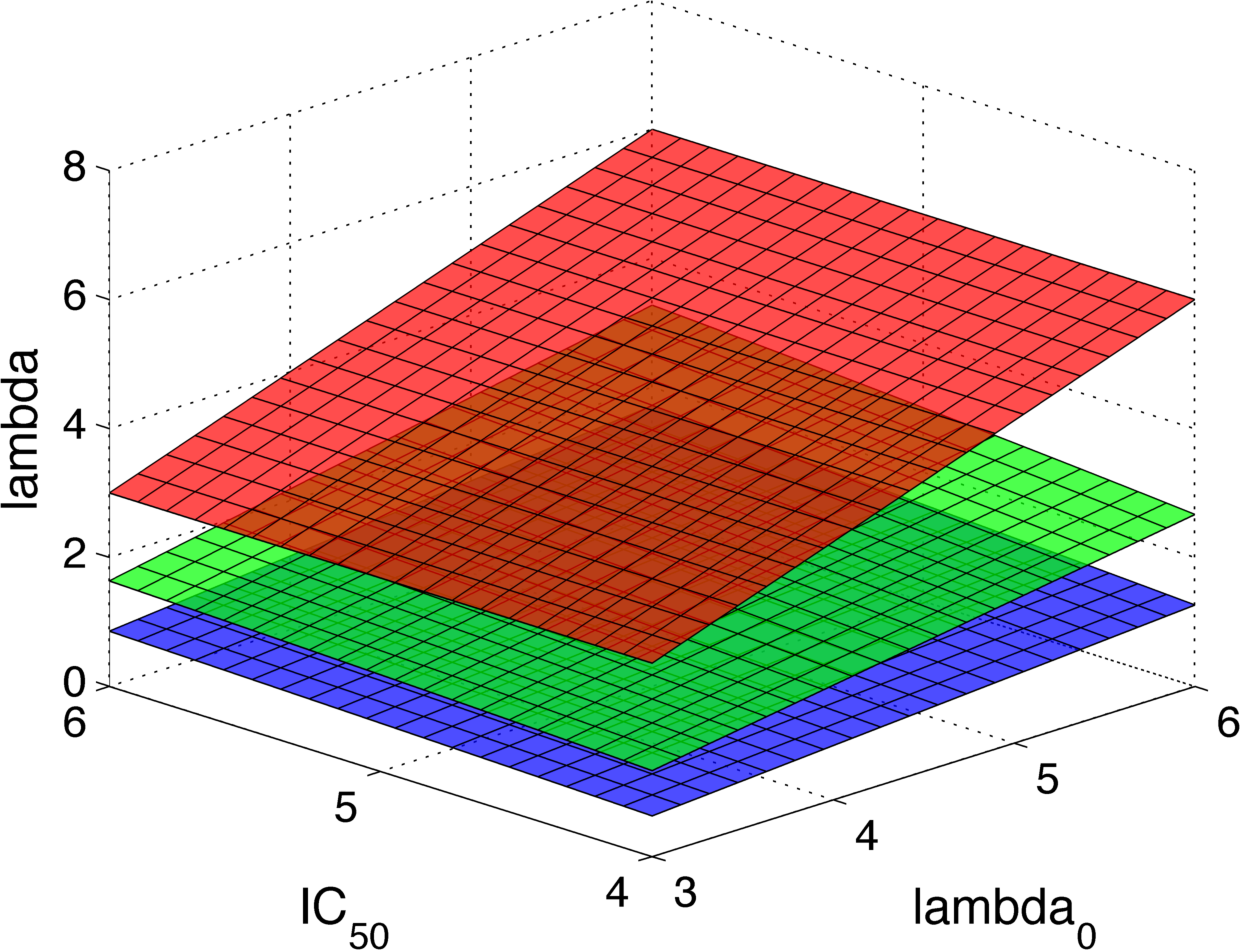
\includegraphics[width=.43\textwidth]{pics/CTS4_lambda_threeSurfaces} 
%& \raisebox{0\height}{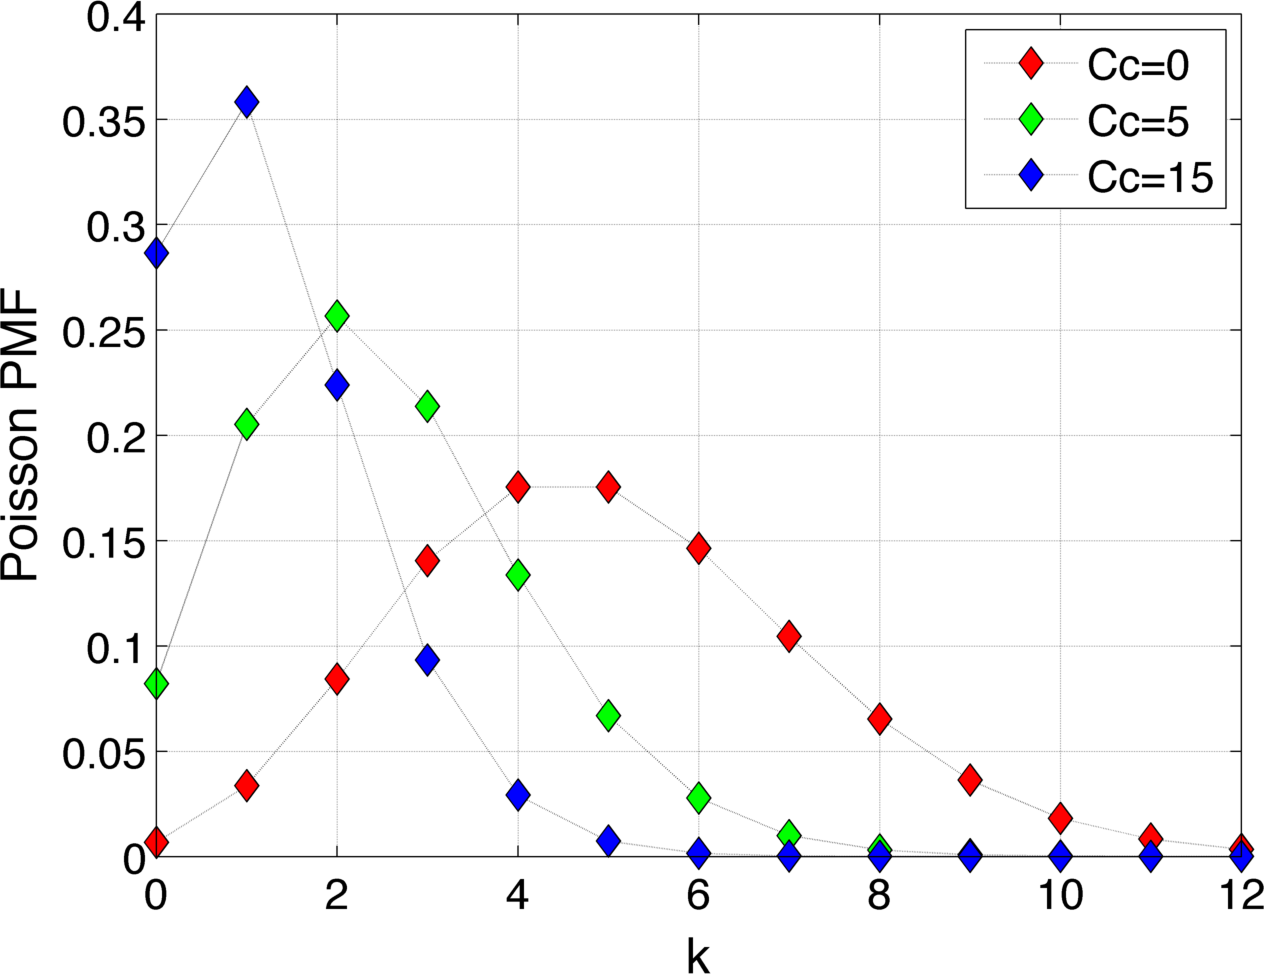
\includegraphics[scale=0.45]{pics/CTS4_poissonScan}}
%\end{tabular}
\caption{$\lambda$--surface as function of $\lambda_0$ and $IC_{50}$ 
plotted for $\Cc = \{1,5,15\}$.}
\label{fig:lambdasurface}
\end{figure}
also called \emph{Poisson intensity}. Here, $\lambda$, depends on the parameters 
$\lambda_0$ and $IC_{50}$ which are sampled from log-normal distribution. 
$\lambda_0$, stands here for the baseline seizure count prior to any drug. 
The value of $\lambda$ is reduced by the concentration in the central 
compartment, $\Cc$, which is visualised for three different values 
of $\Cc = \{1,5,15\}$ in \ref{fig:lambdasurface} ($1\equiv$ green, $5 \equiv$ 
red, $15 \equiv$ blue).


\begin{figure}[ht!]
\centering
\begin{tabular}{cc}
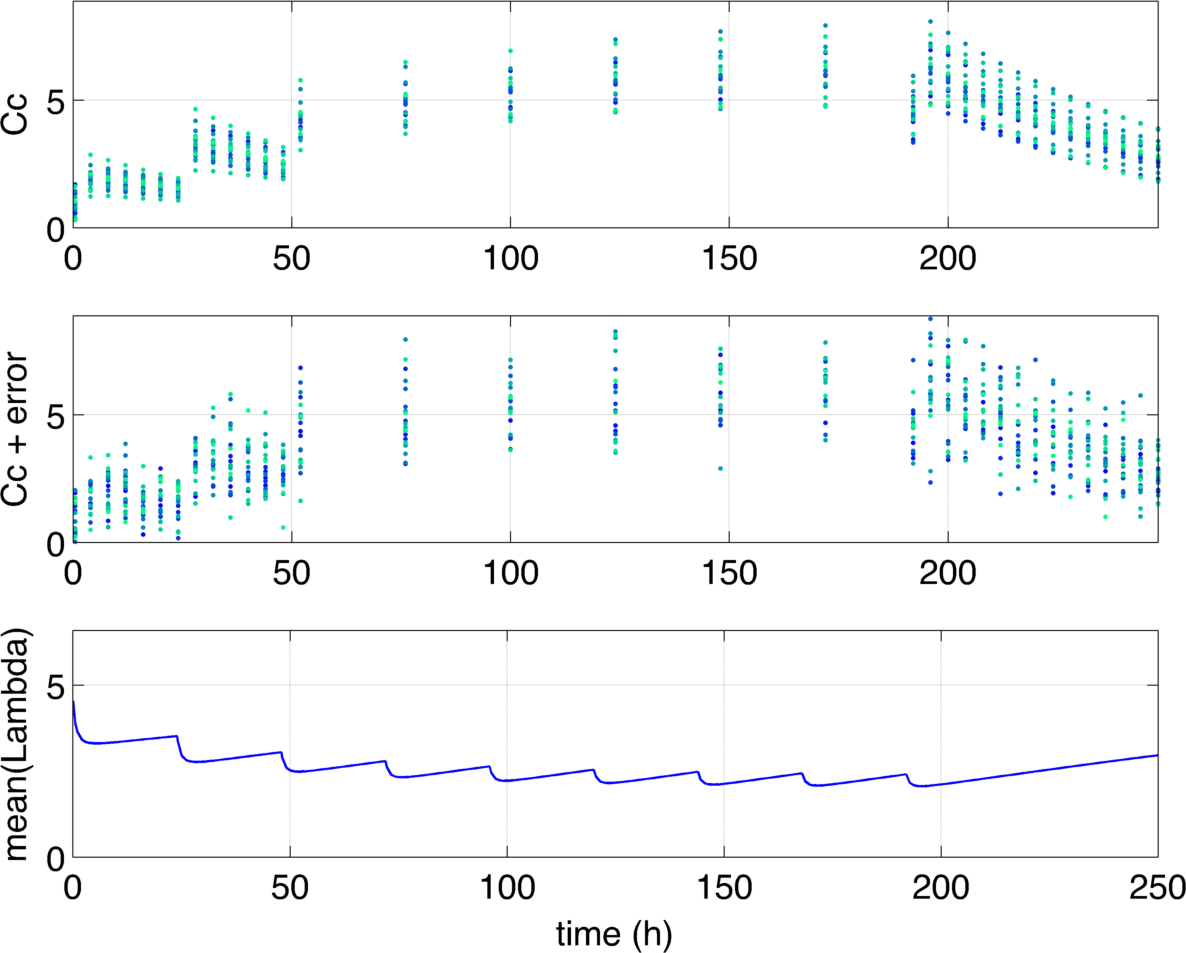
\includegraphics[width=.49\textwidth]{pics/CTS4_PK_meanLambda_armB} & 
\raisebox{0.05\height}{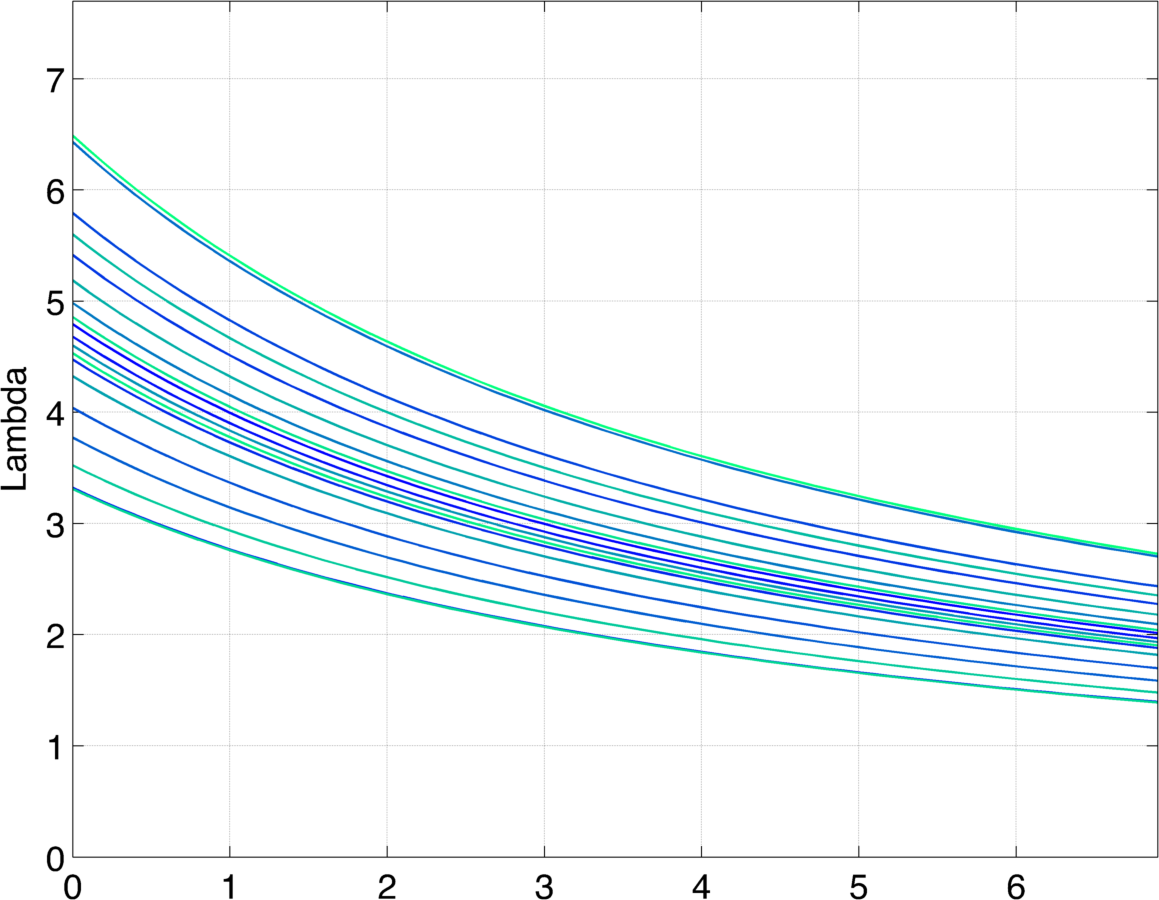
\includegraphics[scale=0.4875]{pics/CTS4_lambda}}
\end{tabular}
\caption{(left) The time courses for the concentration and Poisson intensity. 
(right) Poisson intensity as given by eq.(\ref{eq:lambdasurface}) for all subject as function 
of the concentration between 0 and the maximum concentration in all subjects in the first arm.}
\label{fig:lambdaTiemCourse}
\end{figure}

\subsubsection{Individual parameters model}
\begin{eqnarray}
\lambda_0 & \sim&  \mbox{logNormal}(\pop_{\lambda_0}, \omega_{\lambda_0}); \quad  \pop_{\lambda_0} = 5, \quad \omega_{\lambda_0} = 0.2 \nonumber \\
IC_{50} &\sim& \mbox{logNormal}(\pop_{IC_{50}}, \omega_{IC_{50}}); \quad  \pop_{IC_{50}} = 5, \quad \omega_{IC_{50}} = 0 \nonumber
\end{eqnarray}


\subsubsection{Observation model}
We apply a combined residual error model to the continuous PK output variable 
\var{Cc} and Poisson error distribution for the discrete PD component, defined by \var{Y}, 
as the following table shows 

%\begin{table*}[h!]
\begin{center}
\begin{tabular*}{0.8\linewidth}{@{\extracolsep{\fill}} >{\bfseries}l l l}\toprule
Output Variable & \textbf{\itshape Cc} &\textbf{\itshape Y}\\\midrule
Observation Name & Concentration & State \\
Units & $\mg/l$ & -- \\
Type & Continuous & Discrete/Count \\
Model & Combined & Poisson\\
Parameters 	& $a, b$ 	& $\lambda_0, IC_{50}$\\
%Regressor	& --		& $Cc$ \\
\bottomrule
\end{tabular*}
\end{center}
Two additional important bits of information which are part of the discrete observation
mode to be provided are 
\begin{itemize}
\item
Intensity Parameter, $\lambda$, given by eq. (\ref{eq:lambdasurface})
\item
Link function -- $\log$
\end{itemize}

%%%%%%%%%%%%%%%%%%%%%%%%%%%%%%%%%%%%%%%%%%%%%%%%%%%%%%%%%%%%%%%%
\subsubsection{Modelling Steps}

The PK and PD output variables to be generated by the simulation and
their associated time points are shown below:

\begin{center}
\begin{tabular*}{0.9\linewidth}{@{\extracolsep{\fill}} >{\bfseries}l c c}\toprule
Output Variable & \textbf{\itshape Cc} &\textbf{\itshape $\lambda$}\\\midrule
Observation times & [0.5,4 : 4 : 48, 52 : 24 : 192, 192 : 4 : 250] & 0 : 24 : 192\\
\bottomrule
\end{tabular*}
\end{center}


%%%%%%%%%%%%%%%%%%%%%%%%%%%%%%%%%%%%%%%%%%%%%%%%%%%%%%%%%%%%%%%%
\subsection{Observation model}
While the continuous observation model and its features as applied for example 
for the concentration have been described in very detail in the previous examples,
the error distribution of the discrete effect given by eqs.(\ref{eq:poissonModel}) 
and (\ref{eq:lambdasurface}) will be described in the following for the first time.

First we have to indicate the type of the observation model using the elements 
\xelem{Discrete} and specifically for this example the \xelem{CountData}. The next 
mandatory elements are the count index, \emph{k}, (required only when the PMF is 
explicitly specified, see below) and the \xelem{CountVariable} which will be used later
to establish the link between the model and the related date set, see Table 
\ref{tab:example6_dataSet}.
Then the characteristic parameter for the Poisson distribution is implemented, 
the \emph{Poisson intensity}, $\lambda$, as function of the drug concentration, $Cc$.

\lstset{language=XML}
\begin{lstlisting}
        <ObservationModel blkId="om1">
            <Discrete>
                <CountData>
                    <ct:Variable symbolType="int" symbId="k"/>
                    <CountVariable symbId="Y"/>
                    
                    <!-- Poisson intensity - function of drug concentration, Cc -->                    
                    <IntensityParameter symbId="Lambda">
                        <ct:Assign>
                            <math:Equation>
                                <math:Binop op="times">
                                    <ct:SymbRef blkIdRef="pm1" symbIdRef="lambda0"/>
                                    <math:Binop op="minus">
                                        <ct:Real>1</ct:Real>
                                        <math:Binop op="divide">
                                            <ct:SymbRef blkIdRef="sm1" symbIdRef="Cc"/>
                                            <math:Binop op="plus">
                                                <ct:SymbRef blkIdRef="pm1" symbIdRef="IC50"/>
                                                <ct:SymbRef blkIdRef="sm1" symbIdRef="Cc"/>
                                            </math:Binop>
                                        </math:Binop>
                                    </math:Binop>
                                </math:Binop>
                            </math:Equation>
                        </ct:Assign>
                    </IntensityParameter>
                    <!-- see next listing for the continuation of the observation model -->
\end{lstlisting}
Now the Poisson probability mass function (PMF) can be defined, but here 
in the transformed format 
\begin{align}
\log(P\big(Y_{\iijj} & =k | \Cc_{\iijj}, \psi_i\big)) =  -\lambda_{\iijj} +k\times \lambda_{\iijj} - \log(k!) \nonumber
\end{align}
which can be done in various ways, either
\begin{itemize}
\item
using the UncertML standard as in the following snippet
\lstset{language=XML}
\begin{lstlisting}
                    <PMF linkFunction="log">
                        <PoissonDistribution xmlns="http://www.uncertml.org/3.0" 
                            definition="http://www.uncertml.org/3.0">
                            <rate>
                                <var varId="Lambda"/>
                            </rate>
                        </PoissonDistribution>
                    </PMF>
                </CountData>
            </Discrete>
        </ObservationModel>
\end{lstlisting}
\item
by encoding explicitly the PMF in the transformed format and specifying the
the applied link function, here the logarithm, as the following snippet shows
\lstset{language=XML}
\begin{lstlisting}
                    <PMF linkFunction="log">
                        <math:LogicBinop op="eq">
                            <ct:SymbRef symbIdRef="Y"/>
                            <ct:SymbRef symbIdRef="k"/>
                        </math:LogicBinop>
                        <ct:Assign>
                            <Equation xmlns="http://www.pharmml.org/pharmml/0.6/Maths">
                                <Binop op="minus">
                                    <Binop op="plus">
                                        <Uniop op="minus">
                                            <ct:SymbRef symbIdRef="Lambda"/>
                                        </Uniop>
                                        <Binop op="times">
                                            <ct:SymbRef symbIdRef="k"/>
                                            <Uniop op="log">
                                                <ct:SymbRef symbIdRef="Lambda"/>
                                            </Uniop>
                                        </Binop>
                                    </Binop>
                                    <Uniop op="factln">
                                        <ct:SymbRef symbIdRef="k"/>
                                    </Uniop>
                                </Binop>
                            </Equation>
                        </ct:Assign>
                    </PMF>
                </CountData>
            </Discrete>
        </ObservationModel> 
\end{lstlisting}
\end{itemize}

Note, that although the UncertML driven solution is very simple and straightforward
to implement, it is also limited to only this case, see also Section \ref{subsec:DiscreteData}. 
In short, for count data models, only the basic Poisson model is available in the UncertML standard.


%%%%%%%%%%%%%%%%%%%%%%%%%%%%%%%%%%%%%%%%%%%%%%%%%%%%%%%%%%%%%%%%
\subsection{NONMEM dataset}
\label{sec:eg6-NONMEMdataset}
The remaining part is the the data and trial design as sourced from the 
NONMEM dataset. Table \ref{tab:example6_dataSet} show a typical dataset required for 
an estimation task.
\begin{table}[htdp]
\begin{center}
\small
\begin{tabular}{rrrrrrrr}\toprule
ID 	& TIME	& AMT	& Y		& DVID \\ \midrule
1 	& 0 		& 100 	& . 		& . \\ 
1 	& 4 		& . 		& 9.2 	& 1 \\ 
1 	& 8 		& . 		& 5 		& 2 \\ 
1 	& 12 	& . 		& 8.5 	& 1 \\ 
1 	& 18 	& . 		& 6.4 	& 1 \\ 
1 	& 24 	& . 		& 2 		& 2 \\ 
2 	& 0 		& 120	&  26 	& . \\ 
2 	& 4 		& . 		& 4.8 	& 1 \\ 
2 	& 8 		& . 		& 3 		& 2 \\ 
2 	& 12 	& . 		& 3.1 	& 1 \\ 
2 	& 18 	& . 		& 2.5 	& 1 \\ 
2 	& 24 	& . 		& 0 		& 2 \\ 
...	& ...		& ...		& ...		& ...	\\ \bottomrule
\end{tabular}
\end{center}
\caption{A dataset used in example for first two subjects.
The additional column DVID is used to specify the type of data. Here, 
DVID =1 is used for a continuous response and DVID =2 for count data.}
\label{tab:example6_dataSet}
\end{table}%

\lstset{language=XML}
\begin{lstlisting}
        <mstep:ExternalDataSet toolName="NONMEM" oid="NMoid">
            <mstep:ColumnMapping>
                <ds:ColumnRef columnIdRef="TIME"/>
                <ct:SymbRef symbIdRef="t"/>
            </mstep:ColumnMapping>
            <mstep:ColumnMapping>
                <ds:ColumnRef columnIdRef="AMT"/>
                <ct:SymbRef blkIdRef="sm1" symbIdRef="Ad"/>
            </mstep:ColumnMapping>
            <mstep:MultipleDVMapping>
                <ds:ColumnRef columnIdRef="DV"/>
                <mstep:Piecewise>
                    <math:Piece>
                        <ct:SymbRef blkIdRef="om1" symbIdRef="Y"/>
                        <math:Condition>
                            <math:LogicBinop op="eq">
                                <ds:ColumnRef columnIdRef="DVID"/>
                                <ct:Int>2</ct:Int>
                            </math:LogicBinop>
                        </math:Condition>
                    </math:Piece>
                    <math:Piece>
                        <ct:SymbRef blkIdRef="om2" symbIdRef="Cc_obs"/>
                        <math:Condition>
                            <math:LogicBinop op="eq">
                                <ds:ColumnRef columnIdRef="DVID"/>
                                <ct:Int>1</ct:Int>
                            </math:LogicBinop>
                        </math:Condition>
                    </math:Piece>
                </mstep:Piecewise>
            </mstep:MultipleDVMapping>
            <ds:DataSet>
                <ds:Definition>
                    <ds:Column columnId="ID" columnType="id" valueType="string" columnNum="1"/>
                    <ds:Column columnId="TIME" columnType="idv" valueType="real" columnNum="2"/>
                    <ds:Column columnId="AMT" columnType="dose" valueType="real" columnNum="3"/>
                    <ds:Column columnId="DV" columnType="dv" valueType="real" columnNum="4"/>
                    <ds:Column columnId="DVID" columnType="dvid" valueType="real" columnNum="5"/>
                </ds:Definition>
                <ds:ExternalFile oid="dataOid">
                    <ds:path>datasets/example_poisson.csv</ds:path>
                </ds:ExternalFile>
            </ds:DataSet>
        </mstep:ExternalDataSet>
\end{lstlisting}

Mapping of dosing related data has been described previously on
multiple occasions and will not be discussed here. The conditional mapping required 
in the case when multiple observations have to be mapped using the \xelem{mstep:MultipleDVMapping}
has been described in example 1, see section \ref{sec:eg1-NONMEMdataset}. 
What is new however is the mapping target when dealing with count data.
The count variable, \emph{Y}, as defined in the very beginning of the \xelem{CountData} 
in the observation model \xatt{om1} as the snippet shows
\lstset{language=XML}
\begin{lstlisting}
		<CountVariable symbId="Y"/>
\end{lstlisting}
is the target for this mapping and is conditional on the value of the column \emph{DVID}.




%%%%%%%%%%%%%%%%%%%%%%%%%%%%%%%%%%%%%%%%%%%%%%%%%%%%%%%%%%%%%%%%
%%%%%%%%%%%%%%%%%%%%%%%%%%%%%%%%%%%%%%%%%%%%%%%%%%%%%%%%%%%%%%%%
%%%%%%%%%%%%%%%%%%%%%%%%%%%%%%%%%%%%%%%%%%%%%%%%%%%%%%%%%%%%%%%%

\newpage

\eglabel{7}
\section{Example \theexamples: Joint PKPD model with categorical data}
\label{sec:eg7}

%%%%%%%%%%%%%%%%%%%%%%%%%%%%%%%%%%%%%%%%%%%%%%%%%%%%%%%%%%%%%%%%
\subsection{Description}
\label{subsec:exp7_intro} 
The following example features another type of discrete models supported by \pml -- 
the categorical data models.

In this example, there are two categories, $k \in {0,1}$, i.e. the effect outcome is either 0 or 1. 
The underlying PK model is again an 1-compartmental oral model and will no t be described. 
The probability for the category 1 is given by the following formula 
\begin{eqnarray}
	p1 &=& \frac{1}{1+\exp(-\theta_1 - \theta_2 \log(\Cc))} 	\label{eq:p1surface}
\end{eqnarray}
which is plotted in \ref{fig:p1surface}. This $p1$--surface is also function of $\theta_1$, 
$\theta_2$ and $log(\Cc)$ which is visualised for three different values of $\Cc = \{1,5,15\}$. 

\begin{figure}[htbp]
\begin{center}
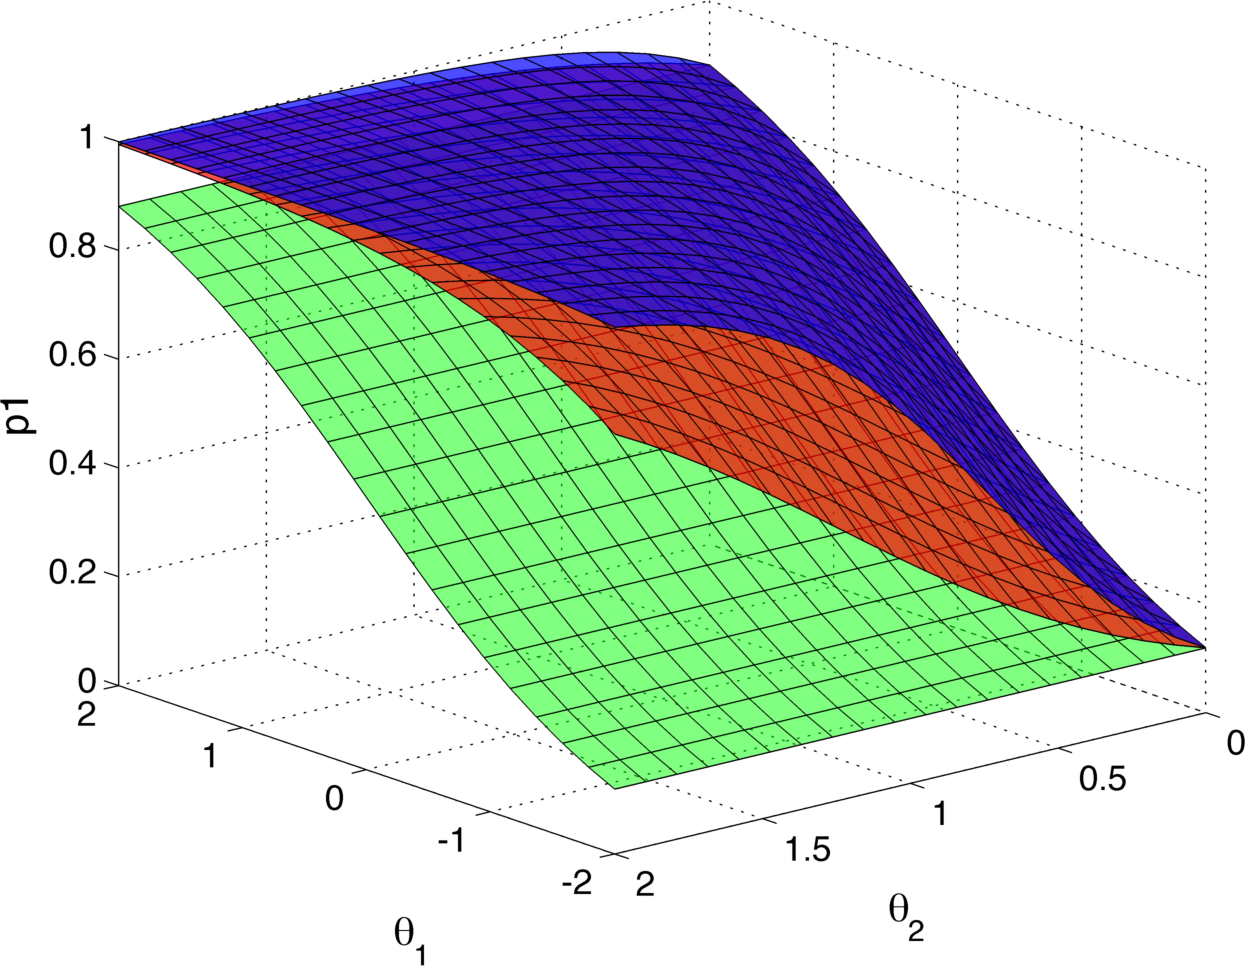
\includegraphics[width=.45\textwidth]{pics/p1_threeSurfaces.png}
\caption{p1 probability surface as function of $\theta_1$ and $\theta_2$ plotted for 
Cc = \{1,5,15\} ($1\equiv$ green, $5 \equiv$ red, $15 \equiv$ blue). }
\label{fig:p1surface}
\end{center}
\end{figure}


\subsubsection{Individual parameters model}
\begin{eqnarray}
theta1& \sim&  \mbox{Normal}(\pop_{theta1}, \omega_{theta1}); \quad \pop_{theta1}=-1,\quad \omega_{theta1}=0.3 \nonumber \\
theta2& \sim&  \mbox{logNormal}(\pop_{theta2}, \omega_{theta2}); \quad \pop_{theta2}=1,\quad \omega_{theta2}=0.2 \nonumber 
\end{eqnarray}

\subsubsection{Observation model}
We apply a combined residual error model to the continuous PK output variable 
\var{Cc} and Poisson error distribution for the discrete PD component, defined by \var{Y}, 
as the following table shows 

%\begin{table*}[h!]
\begin{center}
\begin{tabular*}{0.8\linewidth}{@{\extracolsep{\fill}} >{\bfseries}l l l}\toprule
Output Variable & \textbf{\itshape Cc} &\textbf{\itshape Y}\\\midrule
Observation Name & Concentration & State \\
Units & $\mg/l$ & -- \\
Type & Continuous & Discrete/Categorical \\
Model & Combined & Binomial\\
Parameters 	& $a, b$ 	& $\theta_1$, $\theta_2$\\
%Regressor	& --		& $Cc$ \\
\bottomrule
\end{tabular*}
\end{center}

%%%%%%%%%%%%%%%%%%%%%%%%%%%%%%%%%%%%%%%%%%%%%%%%%%%%%%%%%%%%%%%%
\subsubsection{Modelling Steps}

The PK and PD output variables to be generated by the simulation and
their associated time points are shown below:

\begin{center}
\begin{tabular*}{0.9\linewidth}{@{\extracolsep{\fill}} >{\bfseries}l c c}\toprule
Output Variable & \textbf{\itshape Cc} &\textbf{\itshape $p1$}\\\midrule
Observation times & [0.5,4 : 4 : 48, 52 : 24 : 192, 192 : 4 : 250] & 0 : 24 : 288\\
\bottomrule
\end{tabular*}
\end{center}


\begin{figure}[htbp]
\centering
\begin{tabular}{cc}
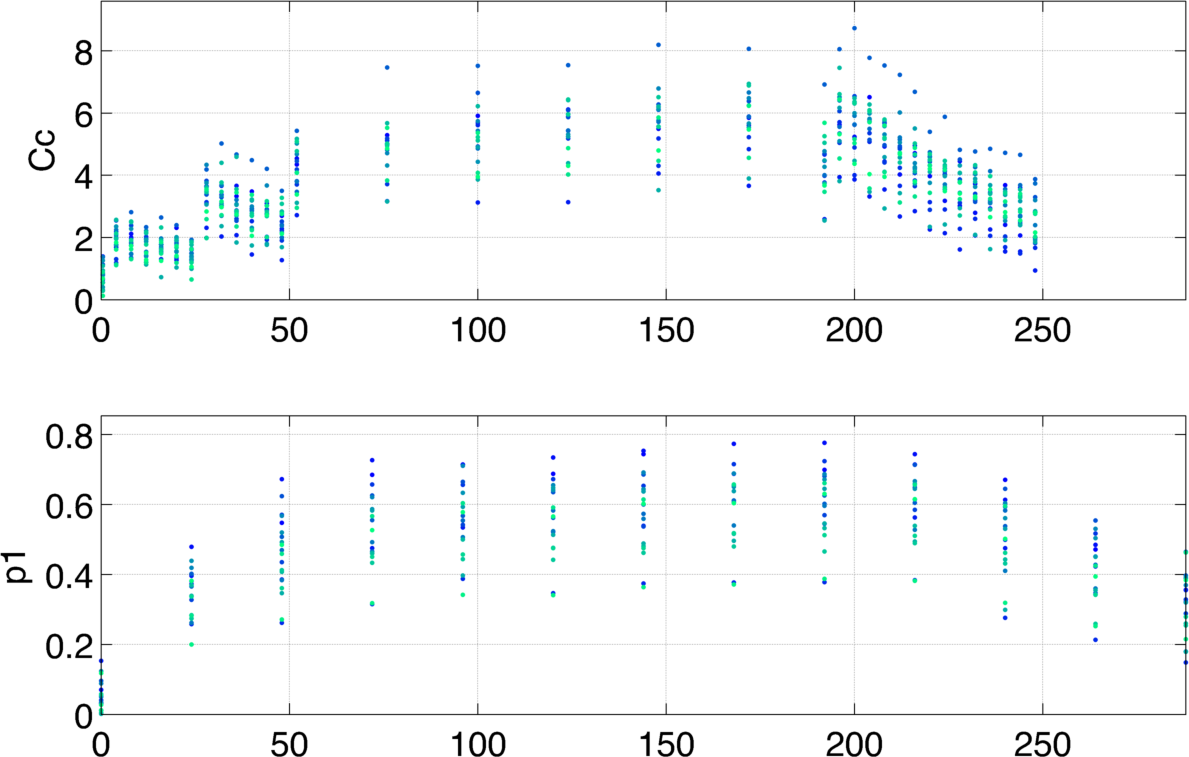
\includegraphics[width=.6\textwidth]{pics/p1_armA} 
\end{tabular}
\caption{Plots for first arm in the study. (top) concentration time course of the PK model. (bottom) Probability \emph{p1}
time course as defined in eq.\ref{eq:p1surface}}
\label{fig:lambdasurface}
\end{figure}


%%%%%%%%%%%%%%%%%%%%%%%%%%%%%%%%%%%%%%%%%%%%%%%%%%%%%%%%%%%%%%%%
\subsection{Observation model}

\lstset{language=XML}
\begin{lstlisting}
        <ObservationModel blkId="om1">
            <Discrete>
                <CategoricalData ordered="no">
                    
                    <ct:Variable symbolType="real" symbId="p1">
                        <ct:Assign>
                            <math:Equation>
                                <math:Binop op="divide">
                                    <ct:Real>1</ct:Real>
                                    <math:Binop op="plus">
                                        <ct:Real>1</ct:Real>
                                        <math:Uniop op="exp">
                                            <math:Binop op="minus">
                                                <math:Uniop op="minus">
                                                    <ct:SymbRef blkIdRef="pm1" symbIdRef="theta1"/>
                                                </math:Uniop>
                                                <math:Binop op="times">
                                                    <ct:SymbRef blkIdRef="pm1" symbIdRef="theta2"/>
                                                    <math:Uniop op="log">
                                                        <ct:SymbRef blkIdRef="sm1" symbIdRef="Cc"/>
                                                    </math:Uniop>
                                                </math:Binop>
                                            </math:Binop>
                                        </math:Uniop>
                                    </math:Binop>
                                </math:Binop>
                            </math:Equation>                            
                        </ct:Assign>
                    </ct:Variable>
                    
                    <ListOfCategories> 
                        <Category symbId="cat0"/>
                        <Category symbId="cat1"/>
                    </ListOfCategories>
                    
                    <CategoryVariable symbId="y"/>
                    
                    <PMF linkFunction="identity">
                        <BinomialDistribution xmlns="http://www.uncertml.org/3.0" definition="">
                            <numberOfTrials>
                                <nVal>1</nVal>
                            </numberOfTrials>
                            <probabilityOfSuccess>
                                <var varId="p1"/>
                            </probabilityOfSuccess>
                        </BinomialDistribution>
                    </PMF>
                </CategoricalData>
            </Discrete>
        </ObservationModel>
\end{lstlisting}

%%%%%%%%%%%%%%%%%%%%%%%%%%%%%%%%%%%%%%%%%%%%%%%%%%%%%%%%%%%%%%%%
\subsection{NONMEM dataset}
\label{sec:eg7-NONMEMdataset}
The remaining part is the the data and trial design as sourced from the 
NONMEM dataset. Table \ref{tab:example7_dataSet} show a typical dataset required for 
an estimation task.
\begin{table}[htdp]
\begin{center}
\small
46	1	1
46	2	0
46	3	0
46	4	0
47	1	0
47	2	0
47	3	0
47	4	3
48	1	0
48	2	1
48	3	2
48	4	0
49	1	0
\begin{tabular}{rrrrrrrr}\toprule
ID 	& TIME	& AMT	& Y		& DVID \\ \midrule
1 	& 0 		& 100 	& . 		& . \\ 
1 	& 1 		& . 		& 1	 	& 2 \\ 
1 	& 4 		& . 		& 9.2 	& 1 \\ 
1 	& 8 		& . 		& 0 		& 2 \\ 
1 	& 10		& . 		& 0	 	& 2 \\ 
1 	& 12 	& . 		& 8.5 	& 1 \\ 
1 	& 18 	& . 		& 6.4 	& 1 \\ 
1 	& 24 	& . 		& 1 		& 2 \\ 
2 	& 0 		& 120	&  26 	& . \\ 
2 	& 4 		& . 		& 4.8 	& 1 \\ 
2 	& 8 		& . 		& 0 		& 2 \\ 
2 	& 12 	& . 		& 3.1 	& 1 \\ 
2 	& 18 	& . 		& 2.5 	& 1 \\ 
2 	& 24 	& . 		& 1 		& 2 \\ 
...	& ...		& ...		& ...		& ...	\\ \bottomrule
\end{tabular}
\end{center}
\caption{A dataset used in example for first two subjects.
The additional column DVID is used to specify the type of data. Here, 
DVID =1 is used for a continuous response and DVID =2 for count data.}
\label{tab:example7_dataSet}
\end{table}%

\lstset{language=XML}
\begin{lstlisting}
        <mstep:ExternalDataSet toolName="NONMEM" oid="NMoid">
            
            <mstep:ColumnMapping>
                <ds:ColumnRef columnIdRef="TIME"/>
                <ct:SymbRef symbIdRef="t"/>
            </mstep:ColumnMapping>
            <mstep:ColumnMapping>
                <ds:ColumnRef columnIdRef="AMT"/>
                <ct:SymbRef blkIdRef="sm1" symbIdRef="Ad"/>
            </mstep:ColumnMapping>
            <mstep:MultipleDVMapping>
                <ds:ColumnRef columnIdRef="DV"/>
                <mstep:Piecewise>
                    <math:Piece>
                        <ct:SymbRef blkIdRef="om1" symbIdRef="y"/>
                        <math:CategoryMapping>
                            <ds:Map dataSymbol="0" modelSymbol="cat0"/>
                            <ds:Map dataSymbol="1" modelSymbol="cat1"/>
                        </math:CategoryMapping>
                        <math:Condition>
                            <math:LogicBinop op="eq">
                                <ds:ColumnRef columnIdRef="DVID"/>
                                <ct:Int>2</ct:Int>
                            </math:LogicBinop>
                        </math:Condition>
                    </math:Piece>
                    <math:Piece>
                        <ct:SymbRef blkIdRef="om2" symbIdRef="C_obs"/>
                        <math:Condition>
                            <math:LogicBinop op="eq">
                                <ds:ColumnRef columnIdRef="DVID"/>
                                <ct:Int>1</ct:Int>
                            </math:LogicBinop>
                        </math:Condition>
                    </math:Piece>
                </mstep:Piecewise>
            </mstep:MultipleDVMapping>
            
            <!-- Dataset omitted, identical as in previous example -->
        </mstep:ExternalDataSet>
\end{lstlisting}



%%%%%%%%%%%%%%%%%%%%%%%%%%%%%%%%%%%%%%%%%%%%%%%%%%%%%%%%%%%%%%%%
%%%%%%%%%%%%%%%%%%%%%%%%%%%%%%%%%%%%%%%%%%%%%%%%%%%%%%%%%%%%%%%%
%%%%%%%%%%%%%%%%%%%%%%%%%%%%%%%%%%%%%%%%%%%%%%%%%%%%%%%%%%%%%%%%

\newpage

\eglabel{8}
\section{Example \theexamples: Joint PKPD model with Time-to-event effect}
\label{sec:eg8}

%%%%%%%%%%%%%%%%%%%%%%%%%%%%%%%%%%%%%%%%%%%%%%%%%%%%%%%%%%%%%%%%
\subsection{Description}
\label{subsec:exp8_intro} 
Time-to-effect is yet another type of discrete models supported by \pml.
In this example we consider a concentration dependent hazard function for which 
the cumulative hazard reads

\begin{eqnarray}
\frac{dCh}{dt} = hazard = \beta \times Cc(t) \quad \Longrightarrow \quad Ch(t) = \beta \int_0^{t} Cc(\tilde{t}) \;d\tilde{t} = \beta \times AUC(Cc(0,t))  \label{eq:hazardODE1}
\end{eqnarray}
The survival function reads, eq.\eqref{eq:survivalFct},
\begin{eqnarray}
S(t) = \exp(-Ch(t)) = \exp(- \beta \times AUC(Cc(0,t))) \label{eq:survivalFct}
\end{eqnarray}

\begin{figure}[htb!]
\centering
\begin{tabular}{cc}
 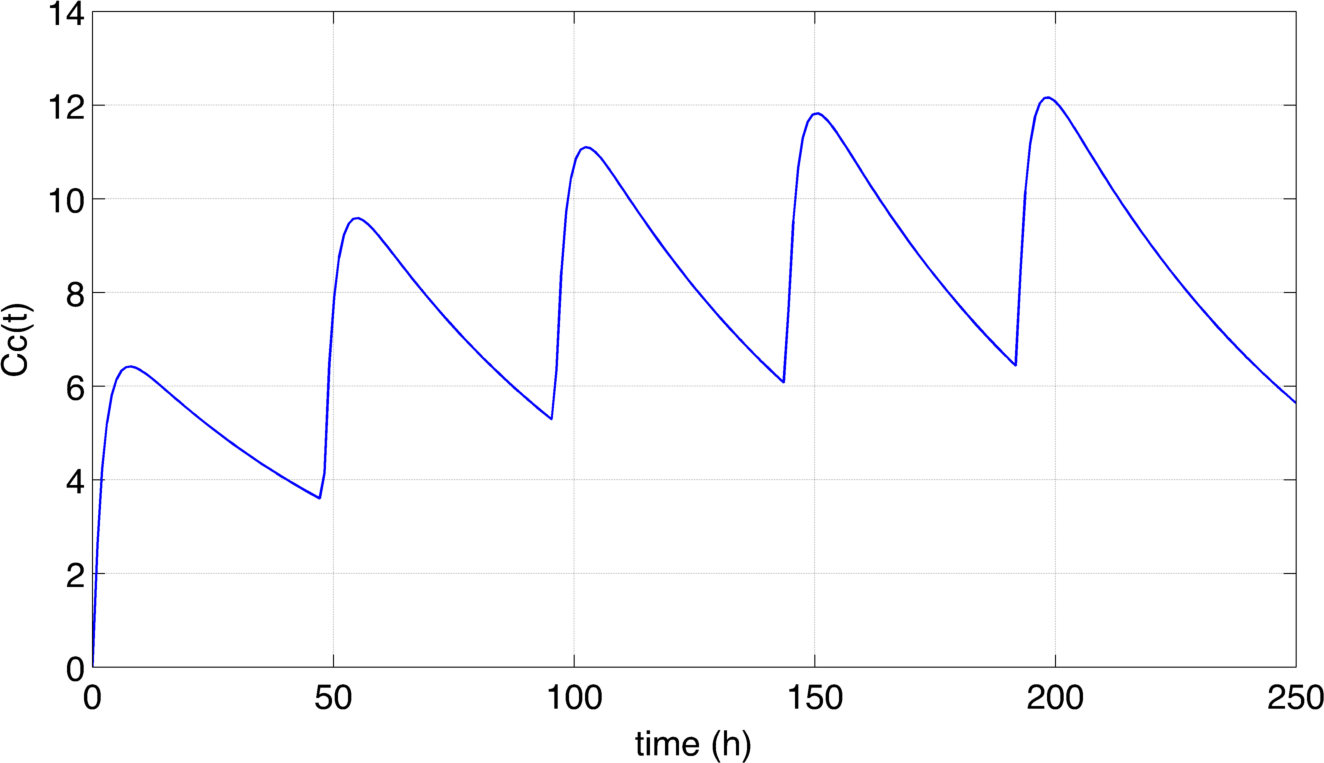
\includegraphics[width=70mm]{pics/example8_singleCc} & 
 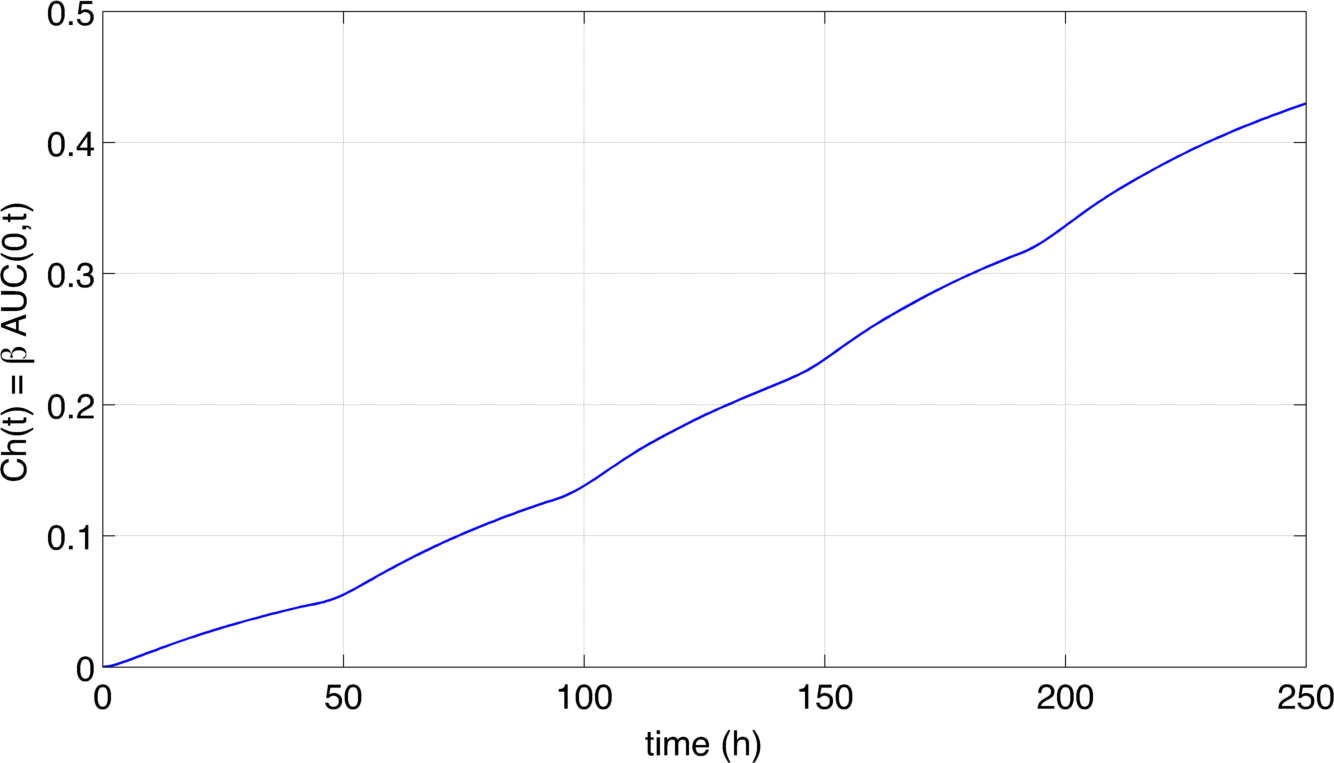
\includegraphics[width=70mm]{pics/example8_singleCh} \\
 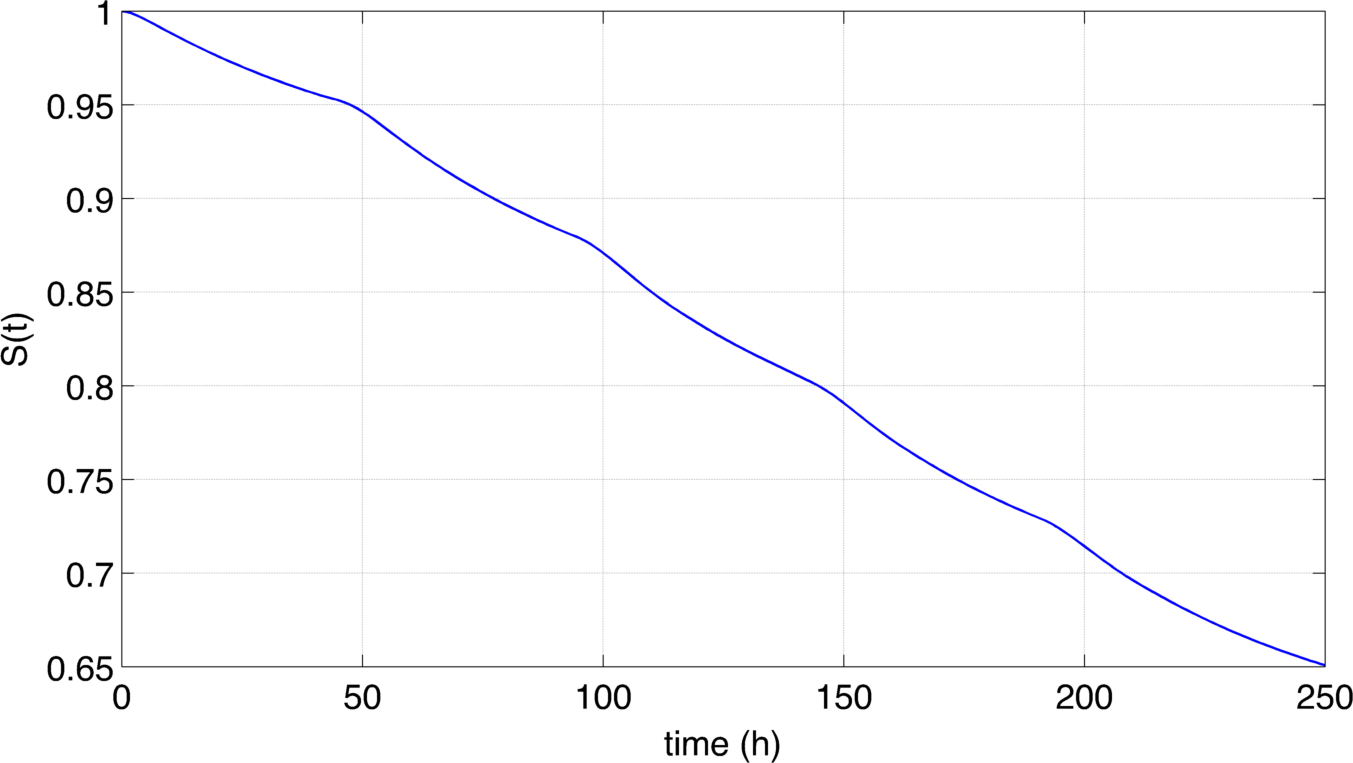
\includegraphics[width=70mm]{pics/example8_singleS} &
\end{tabular}
\caption{Single subject time course for concentration, \emph{Cc}, cumulative hazard, \emph{Ch}, 
and survival function, \emph{S}.}
\end{figure}


\subsubsection{Individual parameters model}
\begin{eqnarray}
beta& \sim&  \mbox{logNormal}(pop_{beta}, \omega_{beta}); \quad \pop_{beta}=0.13,\quad \omega_{beta}=0.2 \nonumber
\end{eqnarray}

\subsubsection{Observation model}
We apply a combined residual error model to the continuous PK output variable 
\var{Cc} and Poisson error distribution for the discrete PD component, defined by \var{Y}, 
as the following table shows 

%\begin{table*}[h!]
\begin{center}
\begin{tabular*}{0.8\linewidth}{@{\extracolsep{\fill}} >{\bfseries}l l l}\toprule
Output Variable & \textbf{\itshape Cc} &\textbf{\itshape Y}\\\midrule
Observation Name & Concentration & State \\
Units & $\mg/l$ & -- \\
Type & Continuous & Discrete/Categorical \\
Model & Combined & Binomial\\
Parameters 	& $a, b$ 	& $\theta_1$, $\theta_2$\\
%Regressor	& --		& $Cc$ \\
\bottomrule
\end{tabular*}
\end{center}
Two additional important bits of information which are part of the discrete observation
mode to be provided are 
\begin{itemize}
\item
Intensity Parameter, $\lambda$, given by eq. (\ref{eq:lambdasurface})
\item
Link function -- $\log$
\end{itemize}

%%%%%%%%%%%%%%%%%%%%%%%%%%%%%%%%%%%%%%%%%%%%%%%%%%%%%%%%%%%%%%%%
\subsubsection{Modelling Steps}

The PK and PD output variables to be generated by the simulation and
their associated time points are shown below:

\begin{center}
\begin{tabular*}{0.9\linewidth}{@{\extracolsep{\fill}} >{\bfseries}l c c}\toprule
Output Variable & \textbf{\itshape Cc} &\textbf{\itshape $p1$}\\\midrule
Observation times & [0.5,4 : 4 : 48, 52 : 24 : 192, 192 : 4 : 250] & 0 : 24 : 288\\
\bottomrule
\end{tabular*}
\end{center}


%%%%%%%%%%%%%%%%%%%%%%%%%%%%%%%%%%%%%%%%%%%%%%%%%%%%%%%%%%%%%%%%
\subsection{Observation model}

\lstset{language=XML}
\begin{lstlisting}

\end{lstlisting}

%\begin{figure}
%\centering
%\begin{tabular}{cc}
% 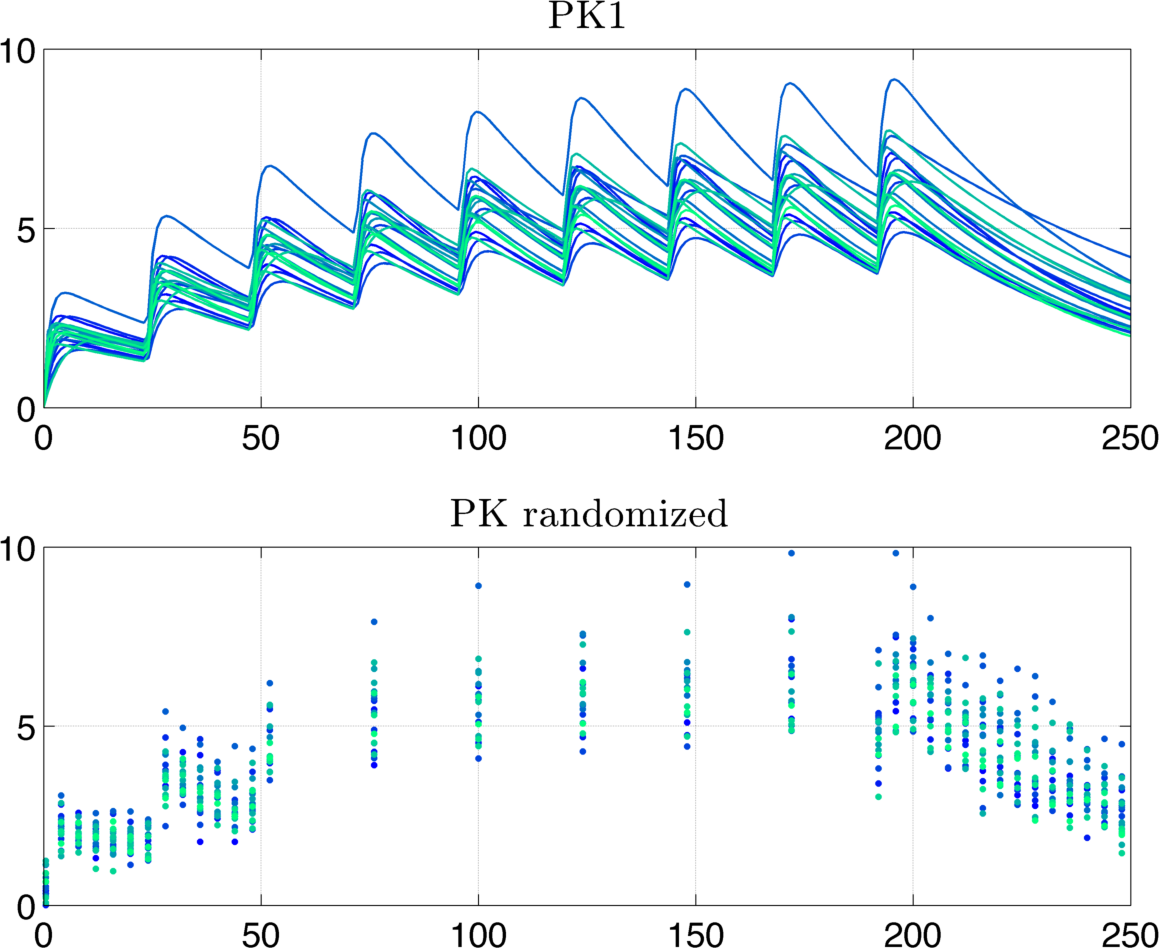
\includegraphics[width=80mm]{pics/example8_PK1_PK2} &
% 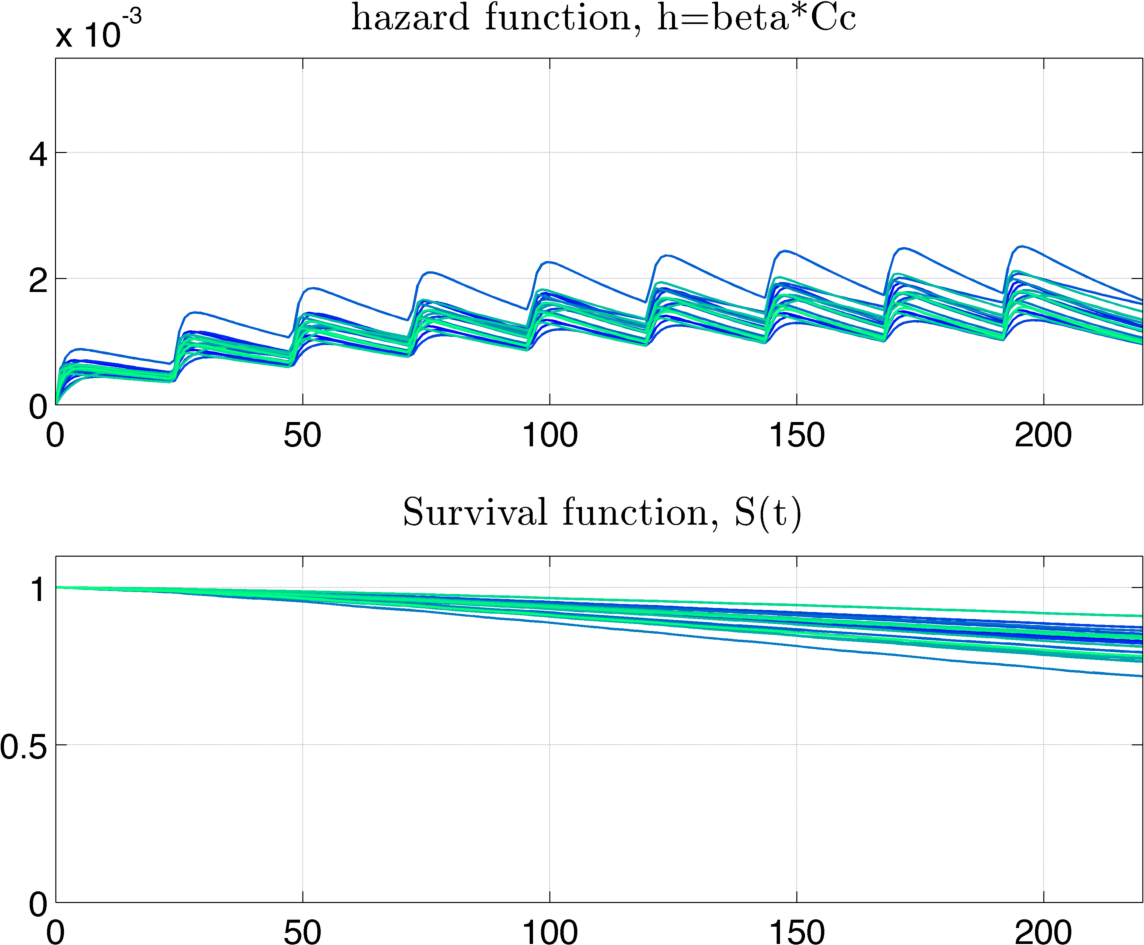
\includegraphics[width=80mm]{pics/example8_hazardPD_S}
%\end{tabular}
%\caption{PK as calculated from the PK model (top left) and with residual error model (bottom left). Hazard and survival function plot, here for arm A (right.)}
%\end{figure}


%%%%%%%%%%%%%%%%%%%%%%%%%%%%%%%%%%%%%%%%%%%%%%%%%%%%%%%%%%%%%%%%
\subsection{NONMEM dataset}
\label{sec:eg8-NONMEMdataset}
The remaining part is the the data and trial design as sourced from the 
NONMEM dataset. Table \ref{tab:example8_dataSet} show a typical dataset required for 
an estimation task.
\begin{table}[htdp]
\begin{center}
\small
\begin{tabular}{rrrrrrrr}\toprule
ID 	& TIME	& AMT	& Y		& DVID \\ \midrule
1 	& 0 		& 100 	& . 		& . \\ 
1 	& 1 		& . 		& 1	 	& 2 \\ 
1 	& 4 		& . 		& 9.2 	& 1 \\ 
1 	& 8 		& . 		& 0 		& 2 \\ 
1 	& 10		& . 		& 0	 	& 2 \\ 
1 	& 12 	& . 		& 8.5 	& 1 \\ 
1 	& 18 	& . 		& 6.4 	& 1 \\ 
1 	& 24 	& . 		& 1 		& 2 \\ 
2 	& 0 		& 120	&  26 	& . \\ 
2 	& 4 		& . 		& 4.8 	& 1 \\ 
2 	& 8 		& . 		& 0 		& 2 \\ 
2 	& 12 	& . 		& 3.1 	& 1 \\ 
2 	& 18 	& . 		& 2.5 	& 1 \\ 
2 	& 24 	& . 		& 1 		& 2 \\ 
...	& ...		& ...		& ...		& ...	\\ \bottomrule
\end{tabular}
\end{center}
\caption{A dataset used in example for first two subjects.
The additional column DVID is used to specify the type of data. Here, 
DVID =1 is used for a continuous response and DVID =2 for count data.}
\label{tab:example8_dataSet}
\end{table}%



